\documentclass{article}
\usepackage{moreverb,code,indent,wrapfig}
\usepackage{makeidx}
\usepackage{times}
\setlength{\topmargin}{-0.4in}
\setlength{\oddsidemargin}{+0.0in}
\setlength{\evensidemargin}{+0.0in}
\setlength{\textheight}{8.5in}
\setlength{\textwidth}{6.50in}
\setlength{\marginparwidth}{0.0in}
\setlength{\marginparsep}{0.0in}
\setlength{\marginparpush}{0.0in}
\setlength{\unitlength}{1.0in}
\setlength{\parskip}{.1in}
\renewcommand{\bottomfraction}{.5}
\renewcommand{\topfraction}{.5}
\usepackage{url}
\usepackage[pdftex]{graphicx}
\pagestyle{headings}
\renewcommand{\baselinestretch}{.95}   % -- double spaced lines
\title{FFS Format Server Administration Guide}
\author{ {\large\bf Greg Eisenhauer }\\
}
\newcommand{\routine}[1]{\index{#1}{\tt #1}}
\makeindex
\makeatletter
\newfont{\titlefont}{cmr17 at 40pt} 
%\newfont{\titlefontb}{ptmr17 at 30pt} 
%\newfont{\titlefontc}{ptmr17 at 20pt} 
\renewcommand\Huge{\@setfontsize\Huge\@xxvpt{30}}
\newcommand{\longpage}{\enlargethispage{\baselineskip}}
\makeatother
\begin{document}
\bibliographystyle{plain}
%uncomment line below
%\maketitle
%recomment lines
\title{FFS Format Server Administration Guide}
\renewcommand{\thepage}{}
\pagenumbering{arabic}
\maketitle
\section{Format server concepts}
All FFS programs that use {\tt FMContext} values communicate with a
third-party {\it format server}.  This format server acts as a repository
for the format information that describes FFS-encoded messages and issues
the format tokens that are prepended to messages in the FFS scheme.  Typical
FFS operation is shown in Figure~\ref{fig:server}.
\begin{figure}[tb]
\begin{center}\
%\psfig{figure=server.eps,width=6.3in}
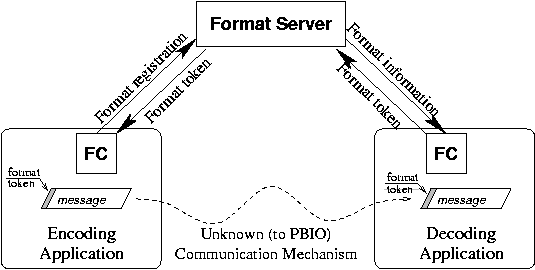
\includegraphics[width=6.3in]{server.png}
\caption{Typical FFS operation.\label{fig:server}}
\end{center}
\end{figure}
The format server may run anywhere in the reachable network.  When encoding
messages applications perform the following basic steps:
In format registration to obtain the format token:
\begin{enumerate}
\item The local format cache is checked to see if the format being
registered is already known.\footnote{I.E. it has already been registered or
an identical format is in the cache for other reasons.  For formats to be
identical all field list entries must be the same, optional information
(such as XML representation) must be identical, and the characteristics of
the registering architecture (pointer size, byte order, floating point
format, etc.) must be the same.}  If the format is known, the format token
is taken from the known format.
\item If there is no current connection to the format server, a TCP/IP
connection is established.
\item An marshalled version of the format information, including full field
lists and native architecture information, is sent to the format server.
\item The application waits on a {\tt read()} call for the return message
from the format server.  The return message contains the assigned format
token.
\item The format information and format token are entered into the local
cache. 
\item The connection to the format server is left open for possible reuse.
The format server may close it asynchronously.
\end{enumerate}
At this point, the format is available for use on the encoding side.  During
encoding, the format token is associated with encoded data.

In the decoding application format information retrieved from the format
server, typically when the incoming buffer is passed to {\tt
get\_format\_FMcontext()} or similar call.  This process follows steps
similar to those in the encoding application, specifically:
\begin{enumerate}
\item The local format cache is checked to see if the format token in the
incoming message is already known.\footnote{I.E. a message of that format
has been seen before or an identical format is in the cache for other
reasons.  In this case only the format tokens of known formats are
compared.}  If the format token is known, the format information associated
with that token is used.
\item If there is no current connection to the format server, a TCP/IP
connection is established.
\item The format token is sent to the format server.
\item The application waits on a {\tt read()} call for the return message
from the format server.  The return message either contains the full format
information that was registered by the encoding application, or it indicates
that the format token is not known.  Among other reasons, the latter
situation might result from attempting to decode a corrupt message, the
encoding and decoding applications using different format servers, or the
format server being restarted since the message was encoded.
\item If format information is retrieved from the format server, the
information and format token are entered into the local cache. 
\item The connection to the format server is left open for possible reuse.
The format server may close it asynchronously.
\end{enumerate}

\section{Behavior of the format server}
The format server is largely a simple database.  It maintains a list of
formats (the full description of a format) and format tokens and searches
one or the other in response to application requests.  The server listens on
a well-known internet port (5347) and waits on messages on its open file
descriptors with a {\tt select()} call.  It allows client applications to
maintain connections, but closes them after they have been idle for one hour
({\tt CONN\_TIMEOUT\_INTERVAL} in {\tt format\_server.c}).  The format
server will also close its oldest connection if it runs out of available
file descriptors.

When the format server accepts a new connection, the connection is
optionally verified against a {\it format service domain}.  This is a simple
security mechanism that allows a format server to limit its service to a
subset of the Internet.  The format service domain value is a
colon-separated list of Internet domain names (such as
``gatech.edu:gt.atl.ga.us'').  This value is set at built time with the
--with-format-server=value argument to configure, or at format server
run-time via the {\tt FORMAT\_SERVICE\_DOMAIN} environment variable.  At
client connection time, the format server will perform a reverse DNS
hostname lookup on the connecting IP address.  If the reverse DNS lookup is
successful and the host falls within one of the service domains, the format
server allows unconditional use.  Otherwise the connecting IP address is
added to a list and use is allowed only for a limited period.  After that,
connections from that IP address will be immediately closed.  This domain
validation can be disabled by defining {\tt FORMAT\_SERVICE\_DOMAIN} as an
empty string.

When registering previously unknown formats, the format server must assign a
new format token.  In the current implementation, format tokens are 10~bytes
long and have the following format:
\begin{verbatim}
typedef struct {
    unsigned char version;
    unsigned char salt;
    unsigned INT2 port;
    unsigned INT4 IP_addr;
    unsigned INT2 format_identifier;
} version_1_format_ID;
\end{verbatim}
The 'version' field is the version of the format token and is '1' for this
format.  'salt' is a random value determined at the time of format server
startup.  It is present simply to aid in the detection of improper or old
format tokens.  'port' is the IP port that the format server is listening on
(currently always 5347).  'IP\_addr' is the IPv4 address of the machine upon
which the format server is running.  'format\_identifier' is a unique value
assigned to each format registered with a particular server.  That
format\_identifier is 16-bits limits the format server to 65536 distinct
formats.  The 'port' and 'IP\_addr' values were added to the format token in
anticipation of supporting multiple interacting format servers.  That
support has not yet been implemented, so these values are not
``operational'' in the sense that they cause FFS to seek out the
appropriate format server.  Instead, the location of the format server is
specified at build time for the FFS library (via the
--with-format-server=value argument to configure).  That value can be
overridden at run-time by specifying the {\tt FORMAT\_SERVER\_HOST}
environment variable.   There is currently no mechanism for customizing the
port that the format server is expected to listen upon.

During normal operation, the format server logs a minimum amount of
information to a text file located at ``/tmp/format\_server\_log''.

\section{Running the format server}

The format server is designed so that it can be easily run automatically
in the background by systems like the Unix cron facility.  To this end, it
is capable of automatically backgrounding itself and disassociating from the
controlling terminal.  When it is run, it first carefully checks to make
sure that there is not already a format server running on its current
machine at its assigned port.   If there is, it exits immediately.  If there
is not it forks a copy of itself into the background.  Most sites run the
format server from cron every 10 minutes to protect against crashes or
reboots. 

The format server accepts the following command line arguments:
\begin{description}
\item[-no\_fork] causes the server to run in the foreground instead of
forking into the background.  This is primarily used for debugging and also
turns out detailed debugging output.
\item[-quiet] suppresses normal startup printouts.  This is useful when
running the format server from cron.
\item[-restart] causes the format server to reload itself with format
information stored in a checkpoint/restart file.  The file's location is
currently hardcoded to be ``/tmp/FS\_restart\_file''.  (Triggering a
checkpoint is discussed in the next section.)
\end{description}
\section{Interacting with the format server}
The format server has some capacity for remote management.  The principal
interface to this is the {\tt format\_cmd} program.  format\_cmd can be used
to check to see if a format server is operational, to dump statistics about
the format server's use, and to cause a checkpoint or restart operation, as
specified below:

\begin{description}
\item[ping] The command line ``format\_cmd ping'' will result in output of
the form ``Format server marquesas.cc.gatech.edu is responsive.'' if the
contacted format server is alive and responding.  Otherwise the response
will be of the form ``Failed to contact format server on host
marquesas.cc.gatech.edu''.
\item[checkpoint] The command line ``format\_cmd checkpoint'' will cause the
format server to checkpoint its current list of formats and format tokens to
the file ``/tmp/FS\_restart\_file''.
\item[restart] The command line ``format\_cmd restart'' will cause the
format server to read the format restart file located at ``/tmp/FS\_restart\_file''.  The format
information there will be added to any formats that are currently known.
Since this is a state-modifying command, this command is only accepted from
clients on the same host as the format server.
\item[stats] The command line ``format\_cmd stats'' will extract statistical
information from the format server and dump it to the standard output.  The
information below is a sample of such output:
\begin{verbatim}

latte% format_cmd stats
Statistics for FFS format server running on marquesas.cc.gatech.edu 
    Server Up Since : Mon Sep 30 12:37:54 2002 
    Known Format Count : 305 
    Test Char Count : 31290 
    Format Registration Count : 16920 
    Format Fetch Count : 15402 
    Client Count (since initiation) : 7140 
    Clients Rejected : 98 
    Current Client Count : 1 
    Stats for client : 
        Client Hostname  : latte.cc.gatech.edu 
        Byte order different : false 
        Provisional Use : false 
        Server Protocol Version  : 2 
        Connected Since : Mon Oct 14 15:47:46 200 
        Bytes received from client : 1 
        Bytes sent to client : 0 
        Number of Formats Registered : 0 
        Number of Formats Fetched : 0 
\end{verbatim}
\end{description}

\section{Environment variables}
Previous sections have discussed the {\tt FORMAT\_SERVER\_HOST} environment
variable that specifies the location of the format server and the {\tt
FORMAT\_SERVICE\_DOMAIN} variable that controls the internet domain freely
serviced by the format server.  In addition, the following environment
variables impact FFS operation in some way.
\begin{description}
\item[FORMAT\_SERVER\_PWD] - When this variable is set to any value, the
format server will substitute the current working directory for '/tmp' as
the location of the format server restart file and the format server log.
\item[FORMAT\_SERVER\_VERBOSE] - When this variable is set for {\it client}
applications (not the format server), those applications will generate
verbose messages describing their interactions with the format server.
\item[FFS\_FIXED\_FORMAT\_IDS] - When this variable is set for {\it client}
applications, they will request and use version-0-style 4-byte format
tokens.  The code that supports older-generation format tokens is no longer
exercised during testing, so this option is deprecated.
\end{description}
\end{document}

# Local Variables:
# latex-run-command:"pdflatex"
# End:
